    \section{Moir\'e materials \& Transition metal dichalcogenides}
    
    Moir\'e materials are two-dimensional heterostructures formed by stacking atomically thin materials, with a small lattice mismatch or a twist angle between them. Due to this misalignment, a spatial interference pattern is formed between the two lattices, which leads to a formation of an artificial crystal with a substantially larger lattice constant --- Moir\'e lattice. In small angle approximation the moire lattice constant is $a_m \approx \frac{a_0}{\theta}$, leading to an increase of the lattice constant by an order of magnitude for typical twist angles of $\theta \in (0, 4^\circ)$.
This in turn leads to effective folding of the Brillouin zone (BZ) of the original material and emergence of Moir\'e bands in the band structure. The separation of length scales between the Moir\'e lattice and the original lattice and the Moir\'e unit cell, leads to a significant enhancement of the effects of interaction relative to the kinetic energy, leading to a plethora of strongly correlated phases of matter.

    Owing to this trait and the unique wide tunability the properties, the field of Moir\'e materials has sparked a revolution in modern condensed matter physics.
    Specifically, the properties can be tuned through:
    \begin{itemize}
        \item A wide choice of constituent 2D materials: graphene, transition metal dichalcogenides (TMDs), transition metal oxides~\cite{li2025twist} and their combinations into multilayer structures
        \item Control over the twist angle between the layers --- changing the Moir\'e lattice constant $a_m$, hybridization between the layers, and in effect the band structure
        \item Strain engineering~\cite{escudero2024designing}
        \item Screening of Coulomb interactions through dielectric environment engineering~\cite{zhao2023probing}
        \item Continuous \textit{in situ} control over the filling of unit cells--- controlling the electron filling of each Moir\'e unit cell
    \end{itemize}

    \begin{figure}[htbp]
        \centering
        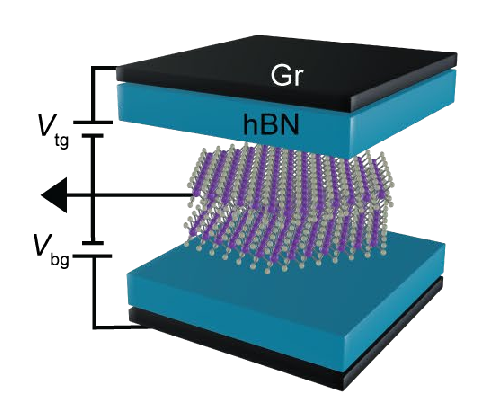
\includegraphics[width=0.5\textwidth]{plots/experimental_setup.png}
        \caption{Experimental setup of a Moir\'e material sandwiched between two spacers and two conducting gates, adapted from~\cite{Cai2023}.}\label{fig:experimental_setup}
    \end{figure}

    The last two points can be easily understood when one considers a typical experimental setup (Fig.~\ref{fig:experimental_setup}), where the material is sandwiched between two spacers and two conducting gates~\cite{Cai2023}. First, the dielectric properties of the spacer, and the distance of the gates from the sample directly affect the screening of electron-electron interactions within the active material. Second, when the gate potential is tuned, due the large periodicity of the material, the electron filling of each Moir\'e unit cell can be easily controlled --- enabling doping by an order of 10 electrons per unit cell.

    \subsection{Transition metal dichalcogenides}
    While the emergence of Moir\'e materials as a prolific research field was catalyzed by the discovery of superconductivity and correlated insulators in twisted bilayer graphene (TBG)~\cite{cao2018correlated, cao2018unconventional}, semiconductor materials joined the field soon after~\cite{mak2022semiconductor}. One of the important features of Moir\'e materials is the emergence of flat bands caused by the large lattice constant of Moir\'e lattice and folding of the brillouin zone --- effective confinement of electrons and suppression of the kinetic energy. However, in heterostructures made from graphene --- described by massless Dirac fermions~\cite{novoselov2005two} (no energy gap) --- the flat bands emerge only at special ``magic'' angles. On the other hand, in semiconductors due to their non-zero bandgap, the condition is relaxed~\cite{wu2018hubbard}. While magic angles can still be identified~\cite{devakul2021magic}, the material is gapped over a wide range of angles and the angle can be continuously tuned. In this class of materials, homobilayers of transition metal dichalcogenides (TMDs) are of particular interest due to
    \begin{itemize}
        \item Relatively simple structure (two layers of the same material)
        \item Relatively low disorder densities
        \item Direct bandgap
        \item Spin-valley locking~\cite{mak2022semiconductor}
    \end{itemize}

    \begin{figure}[htbp]
        \centering
        \begin{subfigure}[b]{0.1\textwidth}
            \centering
            
            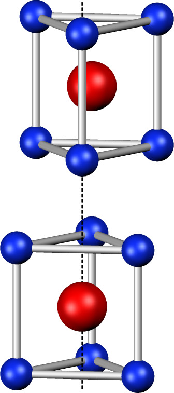
\includegraphics[width=1.0\textwidth]{plots/tmd1.png}
            \subcaption{}\label{fig:tmd_struct1}
        \end{subfigure}
        \hfill
        \begin{subfigure}[b]{0.3\textwidth}
            \centering
            
            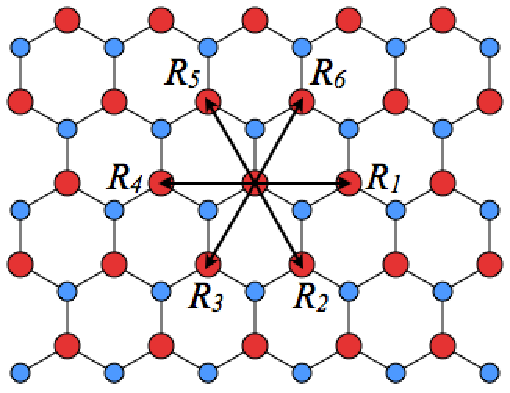
\includegraphics[width=1.0\textwidth]{plots/image8.png}
            \subcaption{}\label{fig:tmd_struct2}
        \end{subfigure}
        \hfill
        \begin{subfigure}[b]{0.4\textwidth}
            \centering
            
            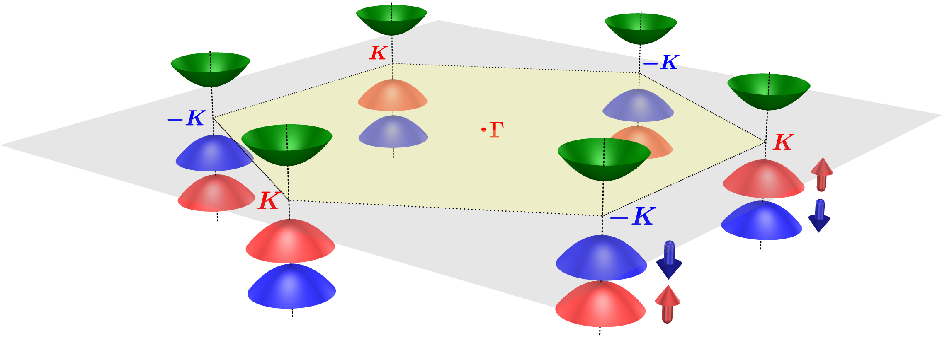
\includegraphics[width=1.0\textwidth]{plots/spin_valley.png}\label{fig:tmd_spin_valley}
            \subcaption{}
        \end{subfigure}
        \caption{Structure of a transition metal dichalcogenide monolayer. (a) Coordination of atoms in a TMD.\@Transition metal (red) is in trigonal prism coordination with chalcogen atoms (blue). (b) Top-view real space structure of a TMD monolayer in 2H phase. (c) Valence band maxima and conduction band minima of a TMD near the K and K' points of the Brillouin zone. Arrows indicate the spin of the electrons.}\label{fig:tmd_general}
    \end{figure}


\begin{figure}[htbp]
    \centering
    \begin{subfigure}[t]{0.55\textwidth}
        \centering
        \includesvg[width=\textwidth]{plots/moire.svg}
        \subcaption{}
        \label{fig:moire_real}
    \end{subfigure}
    \hfill
    \begin{subfigure}[t]{0.4\textwidth}
        \centering
        \includesvg[width=\textwidth]{plots/reciprocal1.svg}
        \subcaption{}
        \label{fig:moire_reciprocal}
    \end{subfigure}
    \caption{TMD --- real and reciprocal space structure, adapted from~\cite{pan2020band}. (a) Real space Moir\'e superlattice of a TMD. The dots in cyan, red and orange indicate $\mathcal{R}_M^M$, $\mathcal{R}_M^X$, $\mathcal{R}_X^M$ local stacking of the atoms (shown in inset). Moir\'e unit cell in blue. (b) Hexagonal Brillouin zone of a metal dichalcogenide monolayer (Red = Top, Blue = Bottom), and a twisted bilayer (Black hexagon), with twist angle $\theta$.}
    \label{fig:moire_structure}
\end{figure}

    TMD monolayers consist of 3 atomic planes --- a middle plane occupied by a transition metal and two outer planes occupied by chalcogen atoms. The two common structural phases are 1T and 2H, from which 2H is the stable one for most of the most commonly studied VI-group TMDs (Fig.~\ref{fig:tmd_struct1}). In 2H phase the transition metal is in a trigonal prism coordination, making up a honeycomb lattice with $\text{D}_\text{3h}$ symmetry (broken inversion symmetry) (Fig.~\ref{fig:tmd_struct2}). Similarly to graphene, the low energy properties can be described in the vicinity of two time-reversal conjugate corners K and -K of the hexagonal 1st Brillouin zone --- the points where the valence band maxima and conduction band minima are located~\cite{coehoorn1987electronic, kormanyos2015k}. It was theoretically modelled by Xiao et al.~\cite{xiao2012coupled} with a two band model, where electrons can be described as massive Dirac fermions. The band structure near the K-points was shown to consist of partially filled d orbitals of the transition metal, with
    \[
     | \phi_c \rangle = | d_{z^2} \rangle, \quad | \phi_v^\tau \rangle = \frac{1}{\sqrt{2}} (| d_{x^2 - y^2} \rangle + i \tau | d_{xy} \rangle)
    \]
    where $\tau = \pm 1$ is the valley index. And $v/c$ subscripts symbolize valence and conduction band respectively. While the conduction band with orbital angular number $L=0$ remains (approximately) spin-degenerate, the valence band built with $L=2$ wavefunctions is split by significant spin-orbit coupling (consequence of broken inversion symmetry), leading to spin-valley locking --- low energy physics of the valence band can be described by a single spin species, with inverse spin in each valley --- thus, the model is time-reversal invariant.
    Due to large distance between valleys in momentum space and due to the spin-valley locking, scattering between the valleys is effectively suppressed. This gives rise to a $U(1) \times U(1)$ symmetry --- charge conservation in each valley, allowing the valley index $\tau$ to be treated as a conserved good quantum number.


    \section{Hall effect and topological order}
        \subsection{Integer Quantum Hall effect}
        \begin{figure}[htbp]
            \centering
            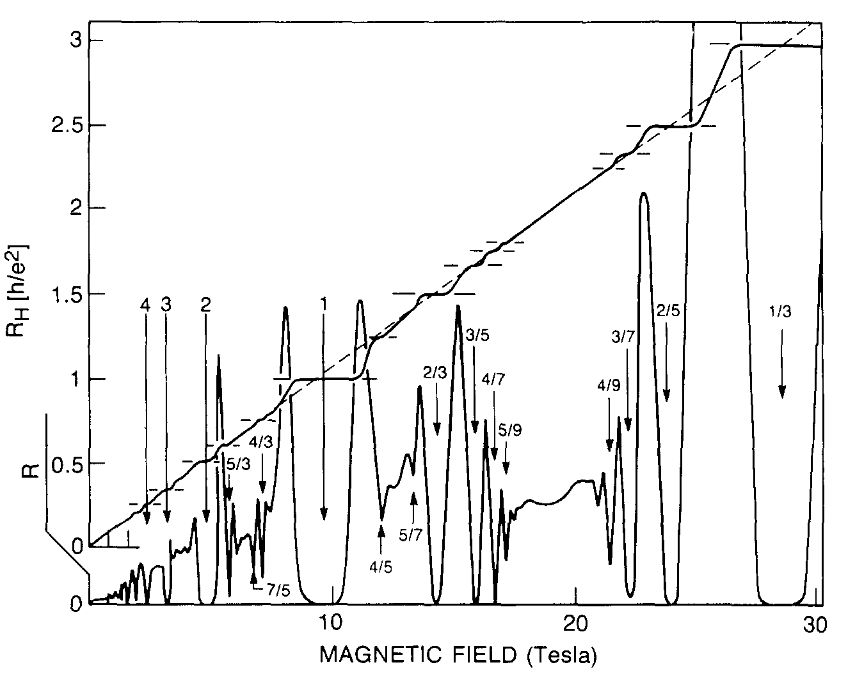
\includegraphics[width=0.5\textwidth]{plots/hall_effect.png}
            \caption{Quantum Hall Effect adapted from~\cite{stormer1992two}.}\label{fig:hall_effect}
        \end{figure}

        The physics of correlated phases in Moir\'e materials has proven in the last years to be very closely related to the physics of the quantum Hall effect --- a phenomenon experienced by a two-dimensional electron system placed in a perpendicular magnetic field, extremely important to the modern condensed matter physics. 
        While classically electrons moving in a 2D system inside a magnetic field simply experience a Lorenz force and and off-diagonal Hall conductivity $\sigma_{xy} \propto B$ can be measured, at low temperatures and in high magnetic fields quantum mechanics comes into play. Quantum mechanically, the magnetic field can be introduced into non-interacting electrons Hamiltonian via the vector potential:
        \[
            \hat{H} = \frac{1}{2m} {\left( \hat{\mathbf{p}} - e \mathbf{A} \right)}^2,\quad B = \nabla \times \mathbf{A}.
        \]
        Introducing appropriate gauge convention (e.g. Landau gauge $\mathbf{A} = (0, Bx, 0)$ or symmetric gauge $\mathbf{A} = (-\frac{1}{2}By, \frac{1}{2}Bx, 0)$), the Schr\"odinger equation can be solved, and the energy spectrum of the system is found to be quantized into equally spaced highly degenerate Landau levels (LLs). The degeneracy, or flatness of Landau levels (LLs) is equivalent to total quenching of the kinetic energy --- similar effect to the one observed in flat Moir\'e bands. This degeneracy of each Landau level is proportional to the number of flux quanta piercing the system, and the filling factor is defined as $\nu = \frac{N_e}{N_\phi}$ where $N_\phi$ is the number of flux quanta and $N_e$ is the number of electrons. In effect, change of the magnetic field changes the filling of LLs.
            Furthermore, via linear response theory, the Hall conductivity can be calculated to take quantized values, dependent directly on the filling $\sigma_{xy} = \nu \frac{e^2}{h},\, \nu \in \mathbb{Z}$, This effect was was discovered in 1980~\cite{von1986quantized} and manifests itself in chracteristic plateaus in the Hall conductivity as a function of magnetic field (Fig.~\ref{fig:hall_effect}). The effect was coined as Integer Quantum Hall Effect (IQHE).
        
        Importantly, physics of IQHE is robust against local disorder and perturbations as it turns out to be topological in nature --- the Hall conductivity can be directly related to the Chern number --- a topological invariant of the system.


        \subsection{Berry phase and Chern number}
        Let
        \[
            \hat{H}(\mathbf{R}(t))
        \]
        be a general Hamiltonian dependent on a time-dependent parameter set $\mathbf{R}(t)$, and
        \[
            \ket{\Psi(0)} = \ket{n(\mathbf{R}(0))}
        \]
        be a non-degenerate eigenstate of the Hamiltonian at time $t=0$, with an energy gap to all other eigenstates.
        The time evolution of the $\ket{\Psi}$ is given by the time-dependent Schr\"odinger equation.
        
        \[
            i \hbar \frac{\partial}{\partial t} \ket{\Psi(t)} = \hat{H}(\mathbf{R}(t)) \ket{\Psi(t)}
        \]
        
        Due to the adiabatic theorem, if the parameters of the Hamiltonian vary slowly enough (with characteristic frequency smaller than the energy gap to other eigenstates), the evolving $\ket{\Psi}$ will remain an instantaneous eigenstate of the Hamiltonian, up to a phase factor
        \[
            \ket{\Psi(t)} = e^{i \gamma(t)} \ket{n(\mathbf{R}(t))}
        \]
        where $\ket{n(\mathbf{R})}$ is the instantaneous eigenstate of the system at time $t$ and $\gamma(t)$ is a phase. Through solving the Schr\"odinger equation, the phase factor is
        \[
            \gamma(t) = -\frac{1}{\hbar} \int_0^t E_n(\mathbf{R}(t')) dt' + \int_{\mathbf{R}(0)}^{\mathbf{R}(t)} \mathbf{A}(\mathbf{R}) \cdot d\mathbf{R}.
        \]

        The first term is a dynamical phase  --- due to the energy of the eigenstate and time evolution itself. The second term is a geometric Berry phase --- it is independent of the time evolution, however, it depends on the path taken in parameter space. The Berry phase can be expressed as a line integral of the Berry connection
        \[
        \mathbf{A}(\mathbf{R}) = i \langle \Psi(\mathbf{R}) | \nabla_\mathbf{R} | \Psi(\mathbf{R}) \rangle
        \]
        Additionally, the Berry curvature is defined as $\mathbf{\Omega}(\mathbf{R}) = \nabla_\mathbf{R} \times \mathbf{A}(\mathbf{R})$.
        Importantly when the path taken in the parameter space is closed, the system returns to its initial state, thus, the Berry phase can only differ by a multiple of $2\pi$. The Berry curvature can be expressed as a surface integral of the Berry curvature over the surface enclosed by the path, $\gamma = \int_S \mathbf{\Omega}(\mathbf{R}) \cdot d\mathbf{S} = 2\pi C$, where $C$ is the Chern number taking integer values. The Chern number is a topological invariant of the system --- since it takes integer values it cannot change continuously, and it can change only when the gap of the system closes. While in general Berry phase is gauge dependent, when the path is closed, Berry phase and thus Chern number are both gauge invariant quantities.. As such it is robust against perturbations. While the notion introduced here is general, in the case of electrons in magnetic field, the Berry curvature corresponds to the magnetic field, the Berry connection to its vector potential, the Berry phase to the Aharonov-Bohm phase and the Chern number to the number of flux quanta piercing the system. Using linear response theory, the Chern number can be shown to be directly related to the Hall conductivity, $\sigma_{xy} = C \frac{e^2}{h}$, so in this case $C = \nu$.~\cite{tong2016lectures}

        These notions can be generalized to treat a degenerate subspace --- the Berry connection becomes a matrix over the degenerate subspace, and the \textit{First} Chern number (which now is one of a bigger group of topological invariants) is defined as $C_1 = \frac{1}{2\pi} \int_S \text{Tr}(\mathbf{\Omega}(\mathbf{R})) \cdot d\mathbf{S}$, where $\mathbf{\Omega}(\mathbf{R}) = \nabla_\mathbf{R} \times \mathbf{A}(\mathbf{R}) - i \mathbf{A}(\mathbf{R}) \times \mathbf{A}(\mathbf{R})$ is the non-abelian Berry curvature.~\cite{tong2016lectures}




        \subsection{Fractional quantum hall effect}
        In clean samples at strong magnetic fields, additional quantum Hall plateaus were detected --- at magnetic fields corresponding to fractional fillings of Landau levels --- effect coined as Fractional Quantum Hall Effect (FQHE) (Fig.~\ref{fig:hall_effect}). While IQHE can be explained by non-interacting electrons, the FQHE is a direct consequence of electron-electron interaction. Such interaction breaks the degeneracy of many-body states within LLs.
        
        Similarly, to IQHE, the FQHE can be related to the (first) Chern number, however the degeneracy of the fractional state has to be taken into account.
        
        The most notable plateaus reside at filling of $\nu = \frac{1}{q}$ with $q \in \mathbb{N_{\text{odd}}}$ (Fig.~\ref{fig:hall_effect}). While an analytical explanation is intractable for Coulomb interaction, an ansatz wavefunction --- Laughlin wavefunction~\cite{laughlin1983anomalous} --- was shown to capture the essential physics. While it is strictly the exact ground state of a simplified pseudopotential Hamiltonian, numerical studies have shown it maintains a remarkably high overlap with the ground states of realistic interactions.

        For such states, and more generally for filling $\nu = \frac{p}{q},\, p\in \mathbb{N},\, q\in \mathbb{N}_{\text{odd}},\,\gcd(p, q) = 1$, due to the algebra of (magnetic translation) operators~\cite{bernevig2012emergent}, the ground state degeneracy is $q^g$ where g is the genus of the manifold under study. A common choice, used also in this thesis, is a torus with $g=1$. Due to the non-abelian Berry connection construction, each of the degenerate states contributes equally to the Chern number and to the Hall conductivity, resulting in the fractional quantization of the Hall conductivity $\sigma_{xy} = \frac{1}{q} \frac{e^2}{h}$ for each of the ground states.
        
        Beyond quantized conductivity, the FQHE is also characterized by the presence of anyonic excitations --- the elementary quasiparticle and quasihole excitations can possess fractional charge (fraction of the charge of an electron), and fractional statistics.
        During a spatial exchange of two quasiparticles, due to their indistinguishability, their wavefunction can only change by a phase factor, $\Psi \to e^{i \theta} \Psi$. For fermions the phase is $\pi$ corresponding to a minus sign, while for bosons the phase is $0$. In 3D, if one particle takes a path around the other and returns to its starting position, the path can be continuously deformed to one where the particle does not move --- thus, double the phase factor has to be a multiple of $2\pi$. However, in 2D this is not the case --- a closed path encompassing another particle is topologically distinct from one that does not encompass any. Thus, the end state need not have the same phase as the starting state, and the exchange phase factor can take any value $\theta \in [0, 2\pi)$. The quasiparticles acquiring this general phase are called abelian anyons.
        However, if the Hilbert space of a single quasiparticle has more than one dimension, the exchange of two quasiparticles can correspond to a more general unitary transformation $\mathbf{U}$ in this local space $\Psi \to \mathbf{U} \Psi$. In this case, the exchange of different particles is non-commutative, and they are \textit{non-abelian} anyons. Since the topological nature of the FQHE is robust against perturbations, the anyonic statistics of the quasiparticles inherits this trait. This makes such topological materials favorable for topological quantum computing --- a notion of using the non-abelian anyons as qubits, where execution of quantum gates would correspond to simple spatial exchanges of the anyons --- ``braiding''~\cite{das2005topologically, nayak2008non}.

        In this aspect, Laughlin states in a FQH system have abelian statistics with the exchange phase $\theta = \frac{\pi}{q}$ for $\nu = \frac{1}{q}$.


\subsection{Composite fermions and the composite Fermi liquid}

    A complementary picture of the fractional quantum Hall effect (FQHE), particularly at even-denominator fillings such as $\nu = \frac{1}{2}$, is provided by composite fermions~\cite{jain1989composite}. In this framework, each electron binds an even number $2p$ of magnetic flux quanta, forming emergent fermionic quasiparticles. This flux attachment can be implemented formally via a singular gauge transformation, providing a mean-field description where the electrons are viewed as composite fermions moving in a reduced effective field
    \begin{equation}
        B_{\mathrm{eff}} = B - 2p\phi_0 n_e,
    \end{equation}
    where $n_e$ is the electron density and $\phi_0 = h/e$ is the flux quantum.
    At filling fractions
    \begin{equation}
        \nu = \frac{p}{2p \pm 1},
    \end{equation}
    the composite fermions fill an integer number of their own effective Landau levels, reinterpreting the FQHE of electrons as an integer quantum Hall effect of composite fermions~\cite{jain1989composite}.

    At the special filling $\nu = 1/2$ (and more generally $\nu = 1/(2p)$), the attached flux effectively cancels the external magnetic field ($B_{\mathrm{eff}} \to 0$), and composite fermions form a compressible, metallic state known as the composite Fermi liquid (CFL). This is confirmed by a definite lack of a plateau in the Hall conductivity at $\nu = 1/2$, in Fig.~\ref{fig:hall_effect}.

        \subsection{Higher Landau levels and non-abelian states}
        While non-abelian states can in principle be found in lowest Landau level, they have been shown to be mostly unattainable with Coulomb interaction\cite{storni2010fractional}. They are, however, found in higher Landau levels e.g. a prominent Hall plateau at $\nu = \frac{5}{2}$ (Fig,~\ref{fig:hall_effect})~\cite{willett1987observation}. 
        As an explanation, an ansatz Moore-Read wavefunction was soon devised~\cite{MOORE1991362}. Like Laughlin wavefunction, it is a ground state of a specific Hamiltonian, however, here the Hamiltonian is composed of 3-body interaction. It was shown numerically to be a good description of the ground state of quantum hall Hamiltonian at $\nu=\frac{5}{2}$. It is worth noting that this notation corresponds not to the half filling of $n=2$ landau level, but to the filling of the lowest Landau level by two spin species, and half filling of the $n=1$ Landau level by one of the species.
        For Coulomb interaction the state is not very robust --- lying close to competing phases --- and the interaction needs to be fine-tuned to stabilize the state~\cite{PhysRevLett.84.4685}.
        
        As Moore-Read state can be understood in terms of Cooper pairing of composite fermions, its ground state degeneracy shows characteristic dependence on the parity of the number of fermions in the system. For a genus $g$ manifold it is shown to be $3(M+1)^g$ for even number of fermions and $3M^g$ for odd number of fermions, where $M$ comes from the filling fraction $\nu=\frac{1}{M+1}$~\cite{bernevig2012emergent}.
        For states studied in the thesis, $g=1$ (torus/PBC) and $M=1\,(\nu=\frac{1}{2})$, expecting degeneracy of 6 and 2 for even and odd number of fermions respectively.~\cite{read2000paired, oshikawa2006fractionalization}

        \subsection{Spectral flow}
        In IQH system with periodic boundary conditions (on a torus), an additional magnetic flux can be inserted into the system through one of the cycles of the torus.
        Such flux insertion affects the energy spectrum of electrons --- effectively modifying the boundary condition while solving for the eigenstates of the system. It can be found, however, that the insertion of an integer number of flux quanta has to leave the spectrum invariant as it can be gauged away. Crucially equality of the spectrum does not mean equality of the eigenstates. Using the magnetic translation operators it was shown that --- the states permute within the degenerate ground state manifold under flux insertion --- a phenomenon called spectral flow.

        The ground state degeneracy and spectral flow were shown to be sufficient conditions to identify a topological nature of phases of matter if the spectral gap does not close in thermodynamic limit~\cite{regnault2011fractional}.


        \section{Topology of Moire materials}

        While the QHE stems from strong magnetic fields, its topological description in terms of Chern number does strictly require them. Impracticality of such strong fields led to a question of whether topological states can be realized in two-dimensional systems without a net magnetic field. First lattice models achieving that~\cite{PhysRevLett.61.2015} introduced explicit time reversal symmetry breaking by introducing a complex hopping term which effectively acts as an analogue of magnetic field and Aharonov-Bohm phase related to it. In result, for a specific parameter range the system's band structure possesses non-zero Chern number. This was later generalized to a more realistic model of graphene~\cite{PhysRevLett.95.226801}. Where the non-trivial hopping amplitude is directly caused by spin-orbit coupling.

        A topologically non-trivial phase with a non-zero Chern number that exhibits the integer or fractional quantum Hall effect without an external magnetic field is known as a Chern Insulator (CI) or Fractional Chern Insulator (FCI), respectively. Although these systems exhibit quantum Hall behavior, they explicitly break time-reversal symmetry. An analogous time-reversal-invariant state can be constructed by combining two time-reversed copies of a Chern insulator with opposite Chern numbers. Because the total Chern number vanishes and time-reversal symmetry is preserved, the net charge Hall conductance is zero. However, if the spin component $s_z$ is a conserved quantity, the system can exhibit a spin quantum Hall effect, where opposite spin channels carry counter-propagating currents with opposite conductances. In the more general case where spin conservation is broken by spin-orbit coupling, the system transitions into a topological insulator (TI), or a fractional topological insulator (FTI).  

    A similar mechanism operates in the effective continuum model of group-VI transition metal dichalcogenides in the $2H$ phase. Near the high-symmetry points $K$ and $-K$, the low-energy physics is described by a massive Dirac Hamiltonian:
    \[
        \hat{H}(\mathbf{k}) = \mathbf{\Delta}(\mathbf{k}) \cdot \mathbf{\hat{\sigma}}
    \]\cite{xiao2012coupled}
    This is analogous to a two-level system in a magnetic field, where the vector $\mathbf{\Delta}(\mathbf{k})$ corresponds to the magnetic field. Here, however, $\mathbf{\Delta}(\mathbf{k})$ acts as a valley pseudospin driven directly by strong spin-orbit coupling.As in the standard description of the Berry phase and Chern number, this two-level Hamiltonian is parametrized by momentum. The Chern number of its eigenstates can be calculated directly by treating the momentum components as parameters. Depending on the sign of the effective mass term, the Chern number of the valence band is $C = \pm 1$ for the $K$ and $-K$ valleys, respectively. In a multi-band continuum model, the global topology of the bands depends strongly on the twist angle. For $\text{MoTe}_2$ at a twist angle of $\theta \approx 1.89^\circ$, for example, it has been found that the two highest occupied bands and the conduction band all possess $C = 1$ and, combined with their flat dispersion, can closely emulate the physics of the three lowest Landau levels~\cite{xu2025multiple, li2025variational}.Consequently, Moir\'e materials provide an exceptionally promising platform for realizing topological phases of matter—including time-reversal-invariant topological insulators and fractional Chern insulators (FCIs) --- by leveraging the presence of two naturally time-reversal-conjugate valleys.
